\section{Second Member}
This is the section dedicated to one of the team members, and it should be written individually . It can include a range of things; first subsection is a space for you to point out the strengths and weaknesses of the module, including complaints about the module coordinator Max Wilson. The second section should have a selfie image with Max! The last part of it is the most important one. You will need to write a paragraph about what you have learned in this module. You can write it in \textbf{Bold} if you want or you can use other fonts. 

Please do not forget:
\begin{itemize}
	\item First paragraph should have your comments about the module
	\item Second one, a selfie img with Max
	\item Last one, what you learned in this module.
\end{itemize}

\subsection{Comments about the module}
G51FSE has been the best few months of my life; everyday I wake up and check my beloved timetable to see if i will be met with joy anytime throughout the day; unfortunately on \textbf{Monday} and \textbf{Wednesday} I am met with gross \textit{dissapointment}, however, to my surprise on any \textit{other day} I stumble upon pure happiness.

Also its quite a lot of theory based content which, \textit{unfortunately} makes most computer science students zone out; but you've done quite well to inject real world examples, and those along with the team exercises seems to keep peoples interest.

\subsection{Selfie with Max}

\begin{figure}[h]
\caption{Selfie with Max}
\centering
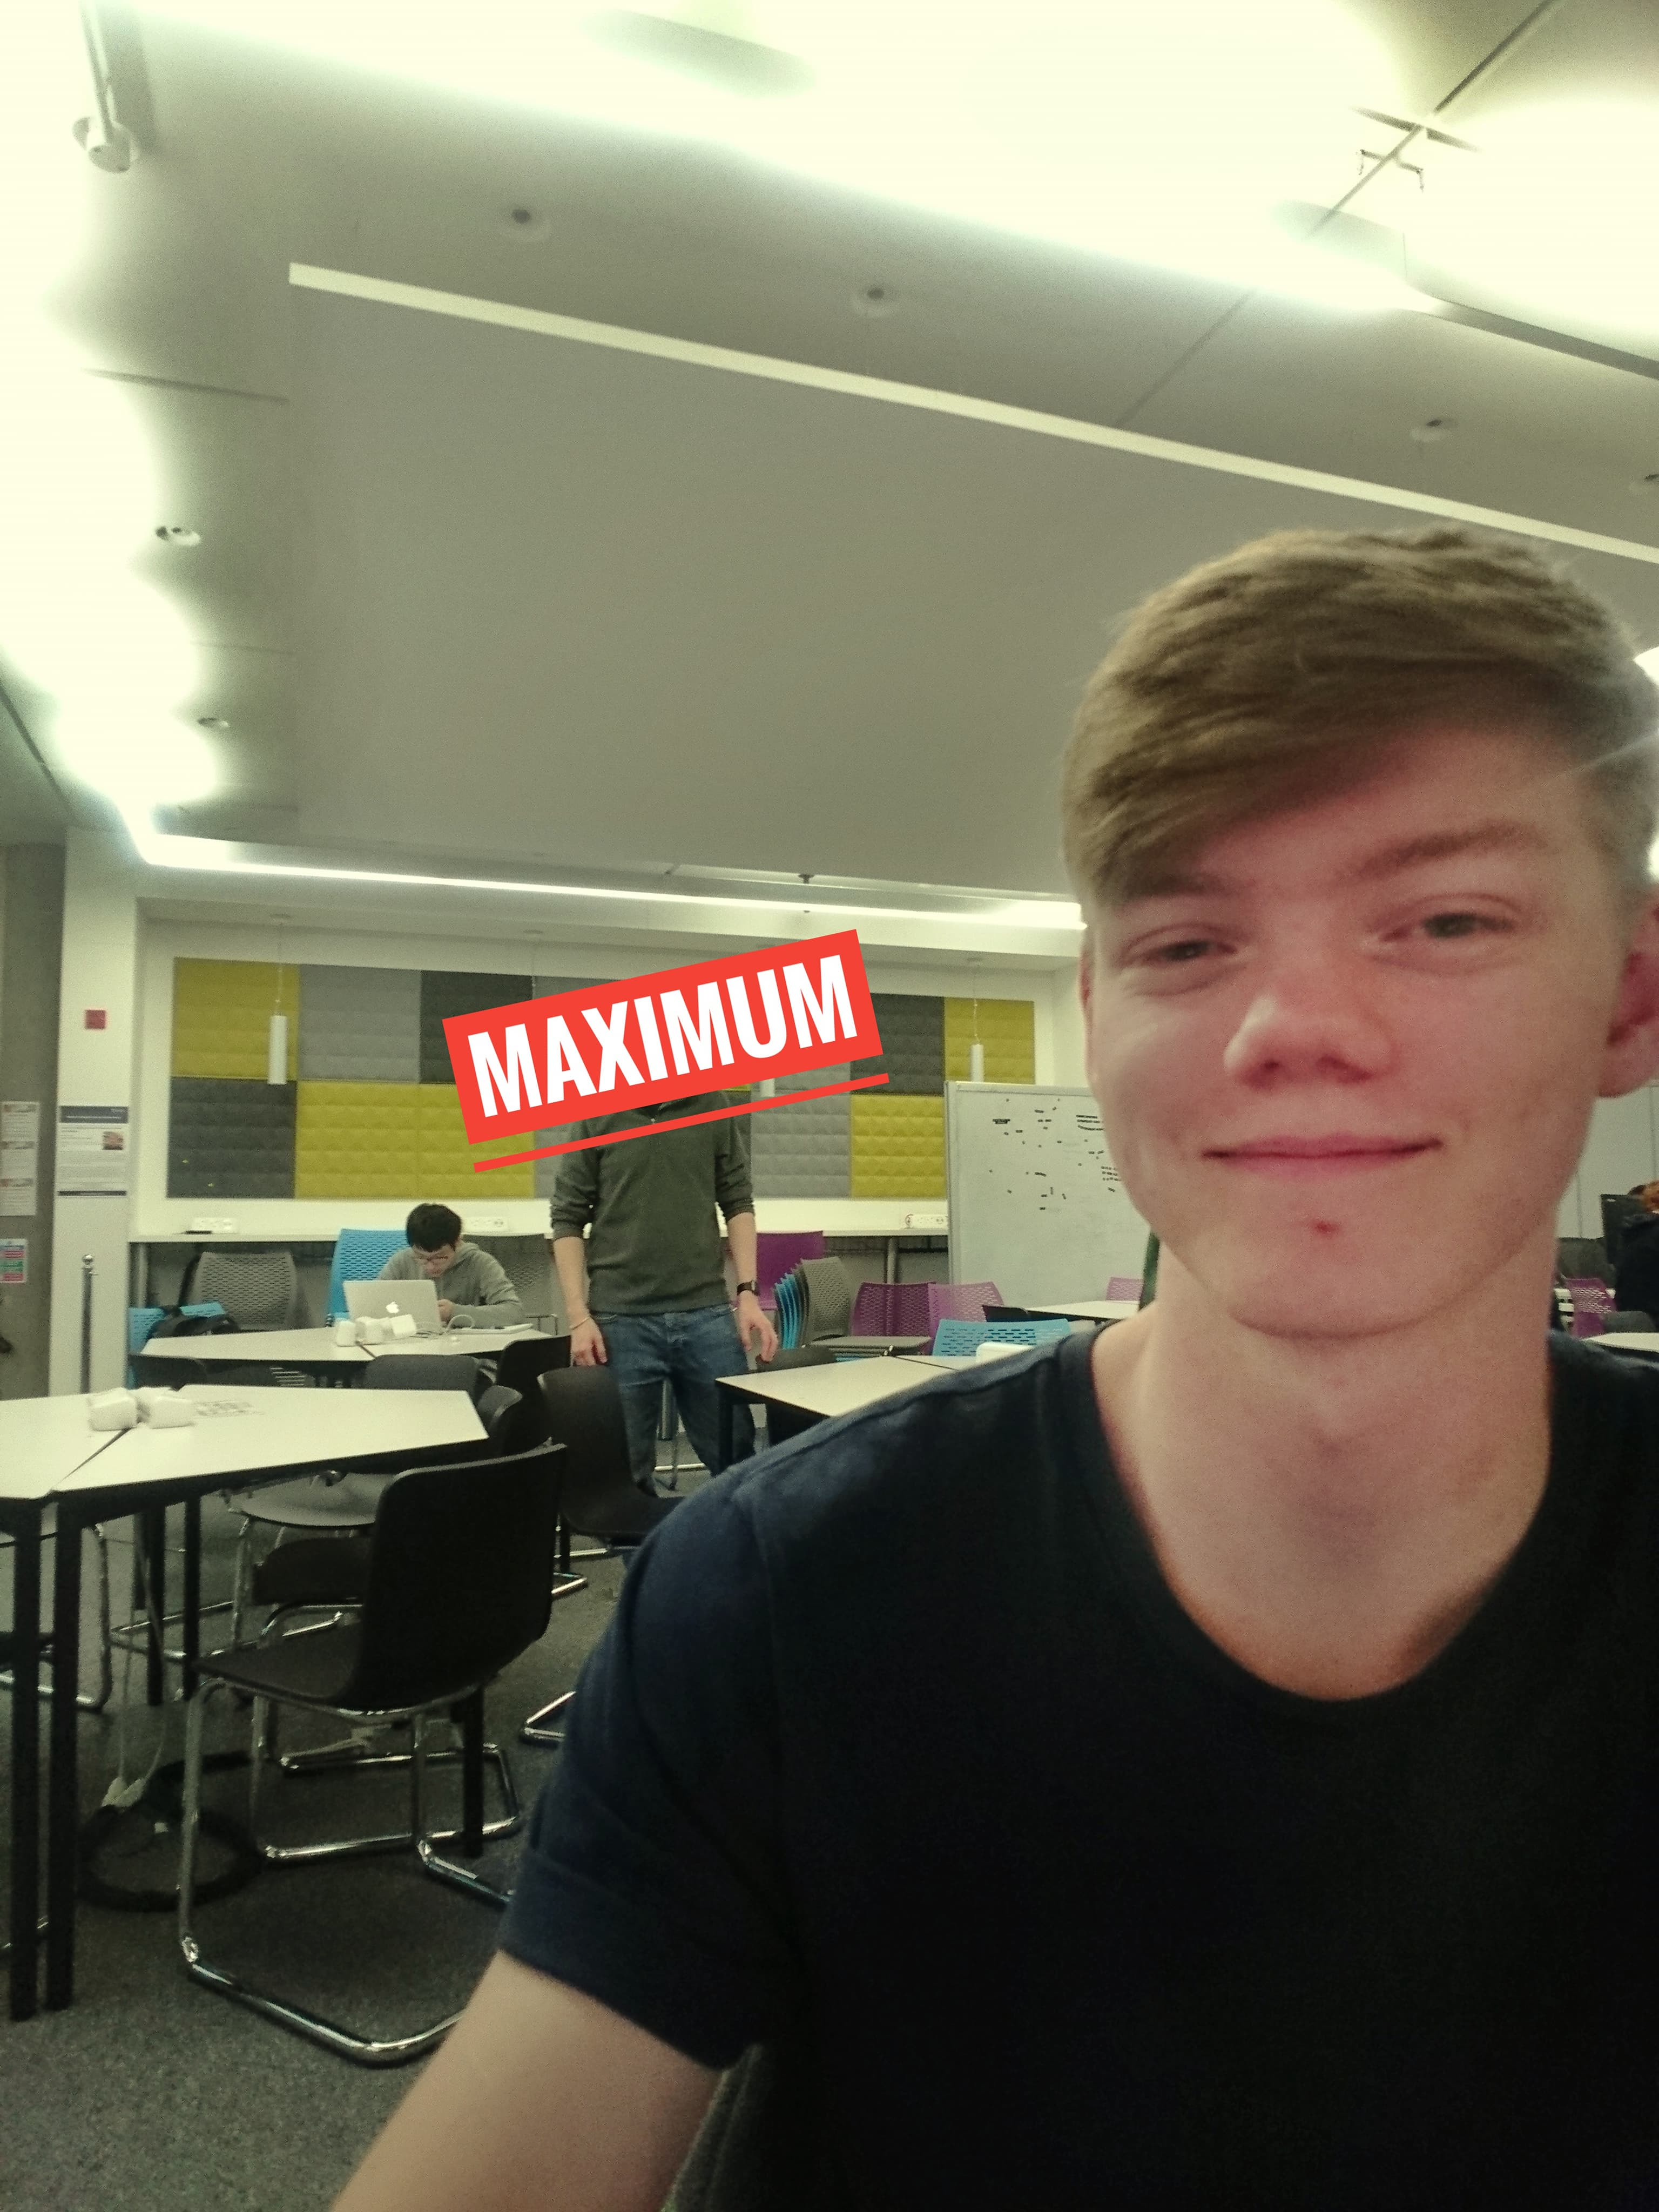
\includegraphics[width=0.5\textwidth]{maxSelfieConnor}
\label{fig:selfie}
\end{figure}


My selfie with Max is in  Figure~\ref{fig:selfie}.

\subsection{What I have learned in this module}
Throughout the last couple of months I have begun to consider the effects my documentation and code style contribute to later \textbf{maintenance} of my projects. It seems apparent that this need for \textbf{clear, transient documentation} is even more important when partaking in \textit{group exercises.}

